\section{Implementation}
In the following section, we describe the implementation specific details of both the simulator as well as the map editing application. We will elucidate problems we faced during the implementation and the integration of both applications and how we solved them. 
\subsection{Simulator}
Behind the user interface of the simulator, a continuously running thread is mandated with updating the current state of the simulation with each tick; every 50ms by default. The thread execution is triggered by the globally governing SimulationController and its \textit{run}-method appears refreshingly simple (fig.~\ref{fig:animthread}). Despite the apparent simplicity, the design of the thread posed a range of problems. As is typical for Java UI frameworks, JavaFX also prohibits changes to UI objects by any thread other the main application thread, forcing us to submit each update that is to be escalated to the interface as a \textit{runnable} object to said application thread's execution queue. To reduce scheduling overhead, we kept the AnimationThread's main loop as simple as possible resulting in no more than four calls to the mentioned execution queue. The calls to \textit{spawnRandomTrucks()} and \textit{spawnRandomCar()} depend on the car/truck-ratio currently observed on the map, i.e. either one of the methods is called depending on the current deviation from the desired ratio. The \textit{updateCharts()} method of the \textit{ControlsController} retrieves the statistics of the simulation from the map and adds a new data point to each of the charts. This is done in 500 millisecond intervals.

\begin{figure}[h]
	\begin{center}
		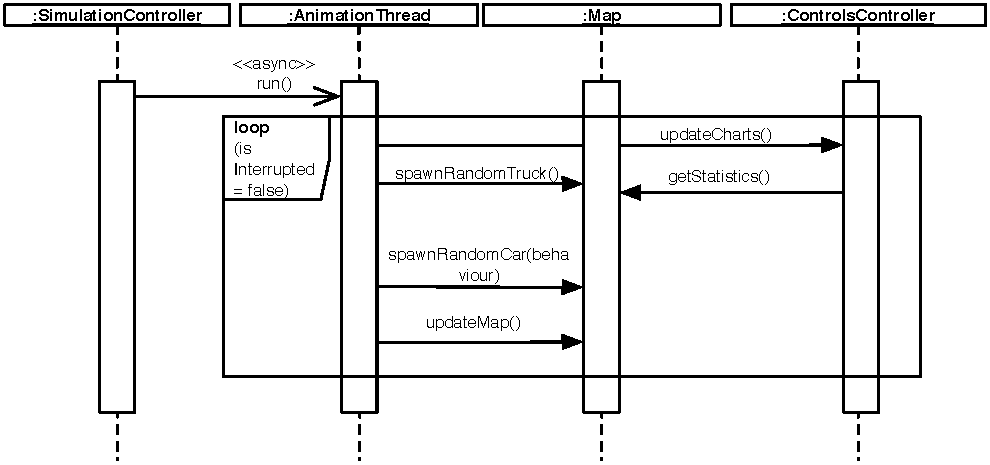
\includegraphics[width=\textwidth]{img/SD_animThread.pdf}
		\caption[Sequence Diagram of the Animation Thread]{Sequence Diagram of the Animation Thread}
		\label{fig:animthread}
	\end{center}

\end{figure}

With the multithreaded execution described above came concurrency related issues. The \textit{Map} class contains a list of all vehicles currently present in the simulation. Whenever a vehicle is leaving the map, it notifies the SimulationController which in turn removes the vehicle from the simulation. Because the map's \textit{updateMap()} method is designed to constantly iterate through its list of vehicles, removing a vehicle from anywhere else other than within this loop results in concurrency exceptions.

\begin{wrapfigure}{r}{0.45\textwidth}
	\begin{minipage}{0.45\textwidth}
		\begin{lstlisting}[caption={Car Removal}, label={lst:carRem}]
if(toBeRemoved.contains(v)){
	iter.remove();
	toBeRemoved.remove(v);
	continue;
}	
		\end{lstlisting}
	\end{minipage}
\end{wrapfigure}

In order to overcome this issue we considered both the traditional reader-writer-locking as well as the more advanced read-copy-update pattern, but eventually came to the conclusion that using either of them will introduce an additional scheduling (and implementation) overhead and hence only yield imperceptible performance improvements over the solution we employed (listing~\ref{lst:carRem}). As mentioned earlier, the \textit{updateMap()} method iterates through all existing vehicles with each tick. During the animation, the map keeps track of vehicles that are about to move off the map within the next tick. As soon as the iterator (\textit{iter}) points to a vehicle \textit{v} that is on the \textit{toBeRemoved} list, it is removed and the loop skips the iteration for this vehicle.

In order to channel the communication between model classes and the \textit{SimulationController} as well as the application classes \textit{MainApp} and \textit{EditorApp} we faced a design decision between the traditional observer pattern and the singleton pattern that allows static access to the required instances. We decided in favour of the singleton pattern, because the situations in which the model communicates with the \textit{SimulationController} are manifold and access to the singleton instance allows for fairly simple flow of communication.

\subsection{Map Editor}

\subsubsection{Graphical User Interface}
The majority of the effort with the editor application was on user interaction (UI) design and implementation. Recall the requirements from \ref{ss:req-editor} particularity those for usability (2.1-2.13). Fig.~\ref{fig:finalMapEditor} shows the resulting design chosen which we felt had met our requirements holistically.


\begin{figure}[h]
	\begin{center}
			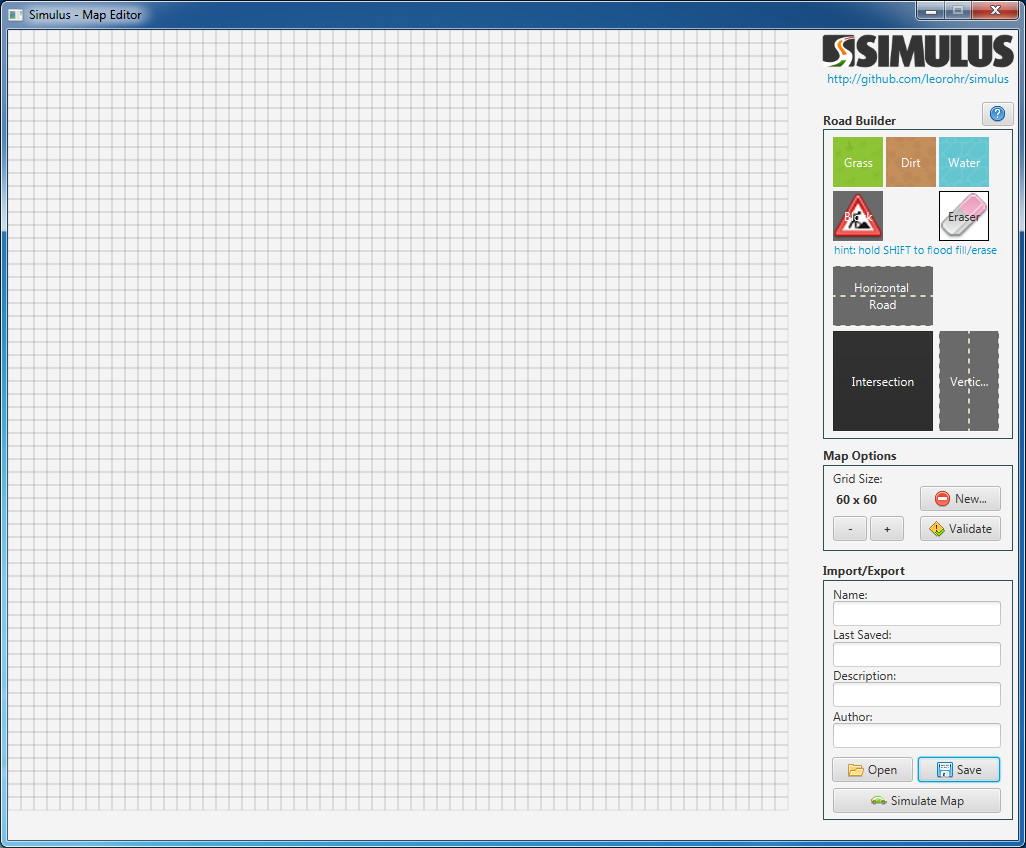
\includegraphics[scale=0.45]{img/mapEditorFinal.png}
		\caption{Resulting map editor design}
		\label{fig:finalMapEditor}
	\end{center}
\end{figure}

\subsubsection{Flood Fill}
The basis of any map editor is the ability to tag defined areas of desktop real-estate representing a real world instance e.g. land mass. We began by constructing an $x*y$ cell grid, where $x$ and $y$ are the number of cells horizontally and vertically and where $x=y$. The smallest instance of a map was to be a 40x40 grid yielding 1,600 tiles each needing to be individually tagged. Clearly, it was not realistic to expect the user to tag each cell individually. Even after accounting for the number of tiles that would be tagged using the road and intersection tools, large swathes of the map are left unfilled.  
For this reason, a method was required that would not only fill the remaining tiles with the users choice of texture but do so intelligently. In other words, the application will only fill empty cells within a certain boundary so as to not replace existing ones. This is is better known as a flood fill algorithm and is listed as requirement 2.7 and 2.8 of section \ref{ss:reqs}

There are several techniques for implementing flood fill of which the 4-way stack based implementation is seen as the simplest and most elegant approach due to its Depth First Search (DFS) recursive property. The appropriate psudocode is as follows:

% probably need a new listing for psudocode?
\begin{minipage}{0.9\textwidth}
	\begin{lstlisting}[caption={4-way stack based recursive flood fill}, label={lst:stackFloodFill}]
Flood-fill (node, target-tile, replacement-tile):
1. If target-tile is equal to replacement-tile, return.
2. If the tile of node is not equal to target-tile, return.
3. Set the tile of node to replacement-tile.
4. Flood-fill (west of node, target-tile, replacement-tile).
   Flood-fill (east of node, target-tile, replacement-tile).
   Flood-fill (north of node, target-tile, replacement-tile).
   Flood-fill (south of node, target-tile, replacement-tile).
5. Return.
	\end{lstlisting}
\end{minipage}

This procedure was extended with bounds checking in our multidimensional array to give the observable results.

\begin{figure}[h]
	\begin{center}
		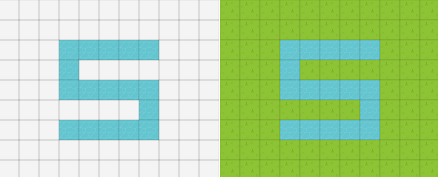
\includegraphics[scale=0.8]{img/floodFill.png}
		\caption[Flood Fill]{Before and after the use of flood fill}
	\label{fig:floodfill}
	\end{center}
\end{figure}

Upon initial testing (ref. jerry's editor testing) the recursive approach performed exactly as expected with no functional issues  to report.  However, when the possibility of larger grid sizes was suggested, further testing revealed a fundamental flaw in this approach.  It was found that for a grid size larger than 65x65, a Stack Overflow error would occur thus only partially filling the grid and causing the application to no longer respond.  With the ability to alter grid sizes implemented in later reversions of the simulator and editor applications, further investigation was warranted.

Approaching the literature, the Stack Overflow observation was commonly experienced and almost expected when using the recursive approach.  Mukherjee and Jana (2010, p.275) emphasise that this error is the most common exception encountered in recursive programs. They explain that when calling a function recursively, the return address, function parameters and local variables are pushed to the stack causing an overflow at times from which there is no recovery.
 
Possibly the simplest but least favoured approach was to alter the JVM's configuration parameters and increase the memory reserved for the stack.  Although this would be the simplest 'fix', it was not seen as a suitable solution given the many hardware and JVM configurations that exist. It simply was not a solution to the fundamental problem at hand.

Ultimately, the the recursive approach was deprecated while a 4-way queue based approach was implemented.  In contrast to the recursive implementation, the queue based method is Breadth First Search (BFS) and uses a queue to store each new encountered tile.  The addition of two checks:

\begin{itemize}
  \item if the adjacent tile in question has not been already visited and
  \item if the tile is not of the target type
\end{itemize}

allowed for a tile to be added to the queue, replaced and dequeued in subsequent iterations. The relevant psudocode for the queue based approach is:

% probably need a new listing for psudocode?
\begin{minipage}{0.9\textwidth}
	\begin{lstlisting}[caption={4-way queue based flood fill}, label={lst:queueFloodFill}]
Flood-fill (node, target-tile, replacement-tile):
 1. If target-tile is equal to replacement-tile, return.
 2. Set Q to the empty queue.
 3. Add node to the end of Q.
 4. While Q is not empty: 
 5.     Set n equal to the last element of Q.
 6.     Remove last element from Q.
 7.     If the tile of n is equal to target-tile:
 8.         Set the tile of n to replacement-tile and mark 
 9			"n" as processed.
 10.        Add west node to end of Q if not yet processed.
 11.        Add east node to end of Q if not yet processed.
 12.        Add north node to end of Q if not yet processed.
 13.        Add south node to end of Q if not yet processed.
 14. Return.
	\end{lstlisting}
\end{minipage}

With this new revised function, grid size was no longer an issue and a flood fill of an empty 200x200 grid (larger than any suggested grid size) completed successfully without any noticeable delay.
\paragraph{}
To ensure the new approach would indeed be suitable for the set grid sizes, some simple measurements were taken. The two algorithms were used to fill an empty grid with a 'grass' type land tile, repeated three times and an average execution time calculated. The results shown in fig.\ref{fig:floodChart} depict clearly that although the recursive stack based implementation performs on average 70\% faster, it was unable to function for grid widths greater than 60 in our set. Although this may seem wholly a failure for the queue based implementation, it is important to point out that this equates to a ~10ms difference; one that is not noticeable by any human operator.  Even more interestingly, the results quoted were based on First Time Run (FTR) values, immediately after launching the editor. Using the same two routines on subsequent occasions would yield repeated values as low as 10-16ms per fill.
 
\begin{figure}[h]
\centering
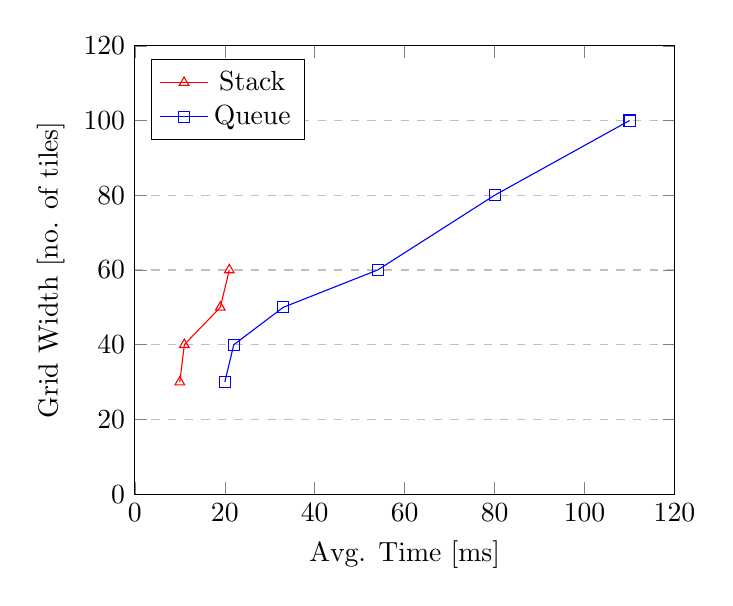
\begin{tikzpicture}
\begin{axis}[
    xlabel={Avg. Time [ms]},
    ylabel={Grid Width [no. of tiles]},
    xmin=0, xmax=120,
    ymin=0, ymax=120,
    xtick={0,20,40,60,80,100,120},
    ytick={0,20,40,60,80,100,120},
    legend pos=north west,
    ymajorgrids=true,
    grid style=dashed,
]
\addplot[
    color=red,
    mark=triangle,
    ]
    coordinates {
    (10,30)(11,40)(19,50)(21,60)
    };
\addplot[
    color=blue,
    mark=square,
    ]
    coordinates {
    (20,30)(22,40)(33,50)(54,60)(80,80)(110,100)
    };
    \legend{Stack, Queue}
\end{axis}
\end{tikzpicture}
\caption{Average execution time for flood fill}
\label{fig:floodChart}
\end{figure}

It must be noted that the new method is no longer as concise as a definition compared to the original but it was a subtle sacrifice for the benefits it yielded.

\subsection{Testing}

An integral part of software development, testing aims to ensure that the original requirements are met. Due to the Agile nature of our development framework, we felt that Feature Driven Development (FDD) is the most adaptable process and well suited for the task at hand. Hence, we decided to test the code iteratively at the end of each development cycle. We came to this decision by foreseeing that the writing of testing code in a concurrent fashion with the development team may not be an effective practice since the implementation was subject to rapid change. Therefore, peer reviews were conducted at an early stage to ensure  code quality is kept to standard, that is, each method should be written explicitly to address the problem that needs to be solved. In such manner, we can be assured of a rigid foundation before we begin to attempt to add more complicated features.

\subsubsection*{Testing Tools}

As the software becomes mature, unit tests were added to the project. We conducted unit testing in JUnit with the support of JemmyFX and ScenicView. JemmyFX is a third party library for testing JavaFX applications. It is a test harness which allows the user to simulate user input such as clicking buttons or entering data. In particular, JemmyFX defines how to get a list of scenes, node items, and the text of a \textit{javafx.scene.control.Label} (listing~\ref{lst:checkBox}). We have mainly used this for UI testing. 


\begin{minipage}{0.9\textwidth}
	\begin{lstlisting}[caption={Use JemmyFX syntax to find a checkBox element}, label={lst:checkBox}]

//Identifying the input checkBox element exist
assertEquals(CheckBox.class, new LabeledDock(scene.asParent(), checkBoxName, StringComparePolicy.EXACT).wrap().getControl().getClass());

//Find the label of the checkBox 
LabeledDock cb = new LabeledDock(scene.asParent(), checkBoxName, StringComparePolicy.EXACT);

	\end{lstlisting}
\end{minipage}

Using ScenicView helped us to understand what the UI was built from, allowing us and any other future developers to quickly and efficiently query the properties of a particular element; easily finding the properties of a JavaFX button (fig.~\ref{fig:scenicview}). ScenicView also provides a tree structure and highlights the item upon selection. this has been particularly helpful in the case of an inability to identify elements within the source code.  
\begin{figure}[h]
	\begin{center}
		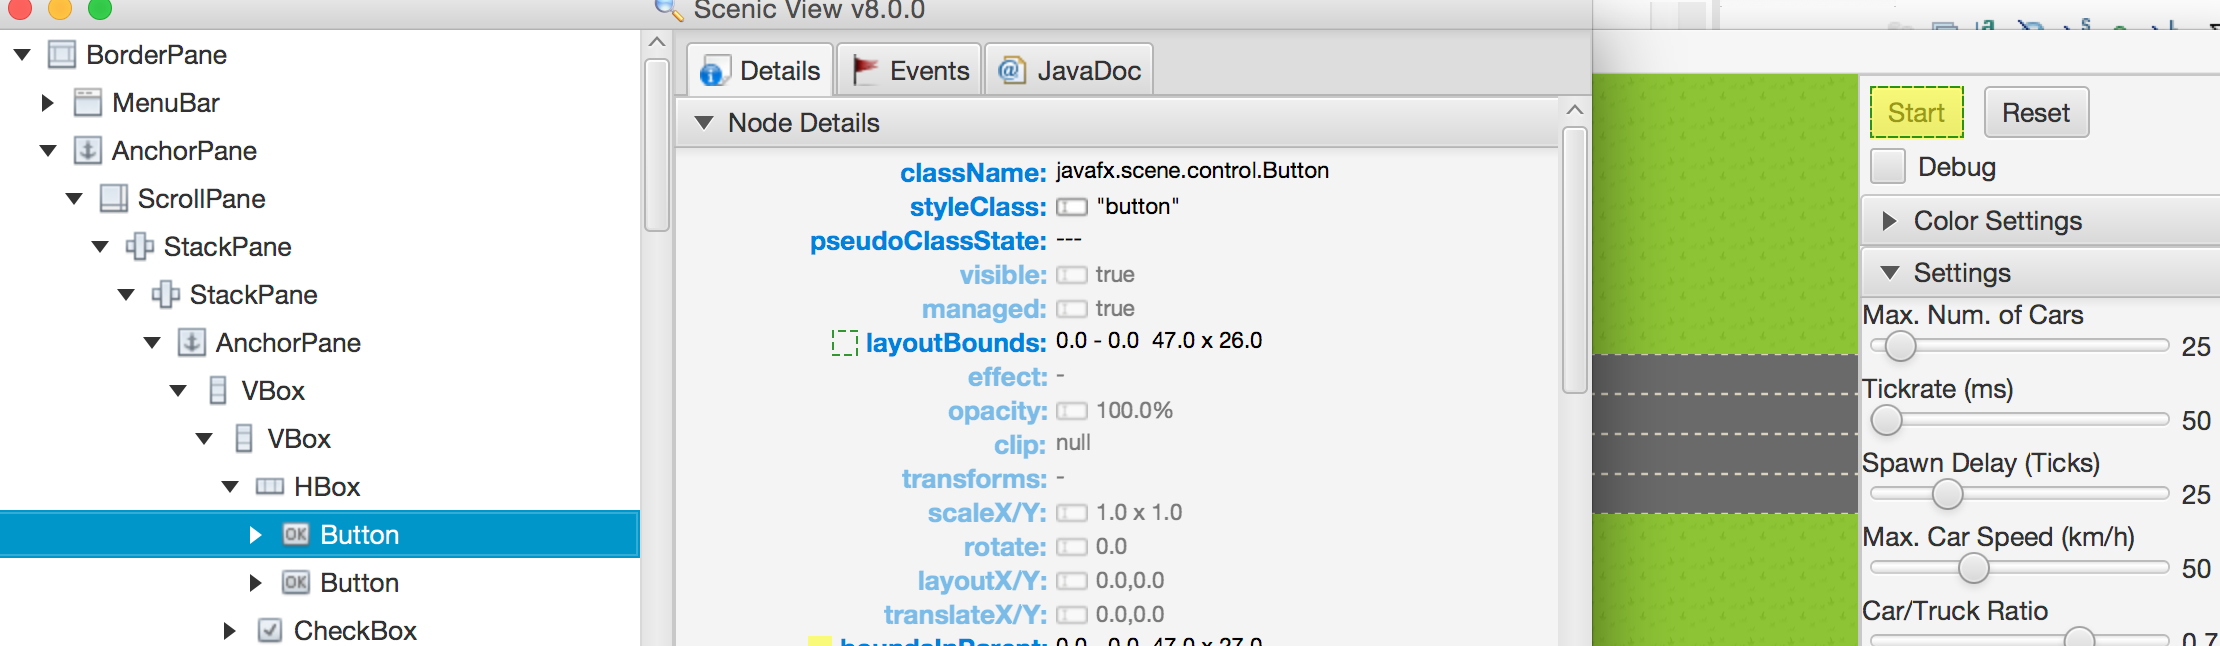
\includegraphics[width=\textwidth]{img/scenicView.png}
		\caption[Identifying properties of Start button with ScenicView]{Identifying properties of Start button with ScenicView}
	\label{fig:scenicview}
	\end{center}
\end{figure}

\subsubsection*{Unit Testing}
Successfully implementing a multi-threaded application, we reached a point where it was very difficult to test all functionality due to the fact that nesting and threading was deep beyond comprehension. We therefore mainly focused our unit testing on major components (i.e. vehicles, map and model), and the components within them with a main driver of ensuring correct functionality. With such an approach, we were given the confidence that the software functioned as required.

As can be expected, large and complex applications require an extensive period of time for thorough testing. In the interest of time, however, achieving absolute branch and statement coverage was not of high priority. Our main concern is to test whether or not the components of the system could work together as a whole.  With this mentality, we carried out tests to ensure that the foundation of our code is dependable based on the requirements. Test cases were developed to be automated, allowing us to reduce the workload on manual testing and easily repeat basic functionality tests. A log was produced at the end for every test scenario enabling us to easily identify problem areas and amend them. An illustration of a testing log is shown in figure ~\ref{fig:testCase}. 

\begin{figure}[h]
        \begin{center}
                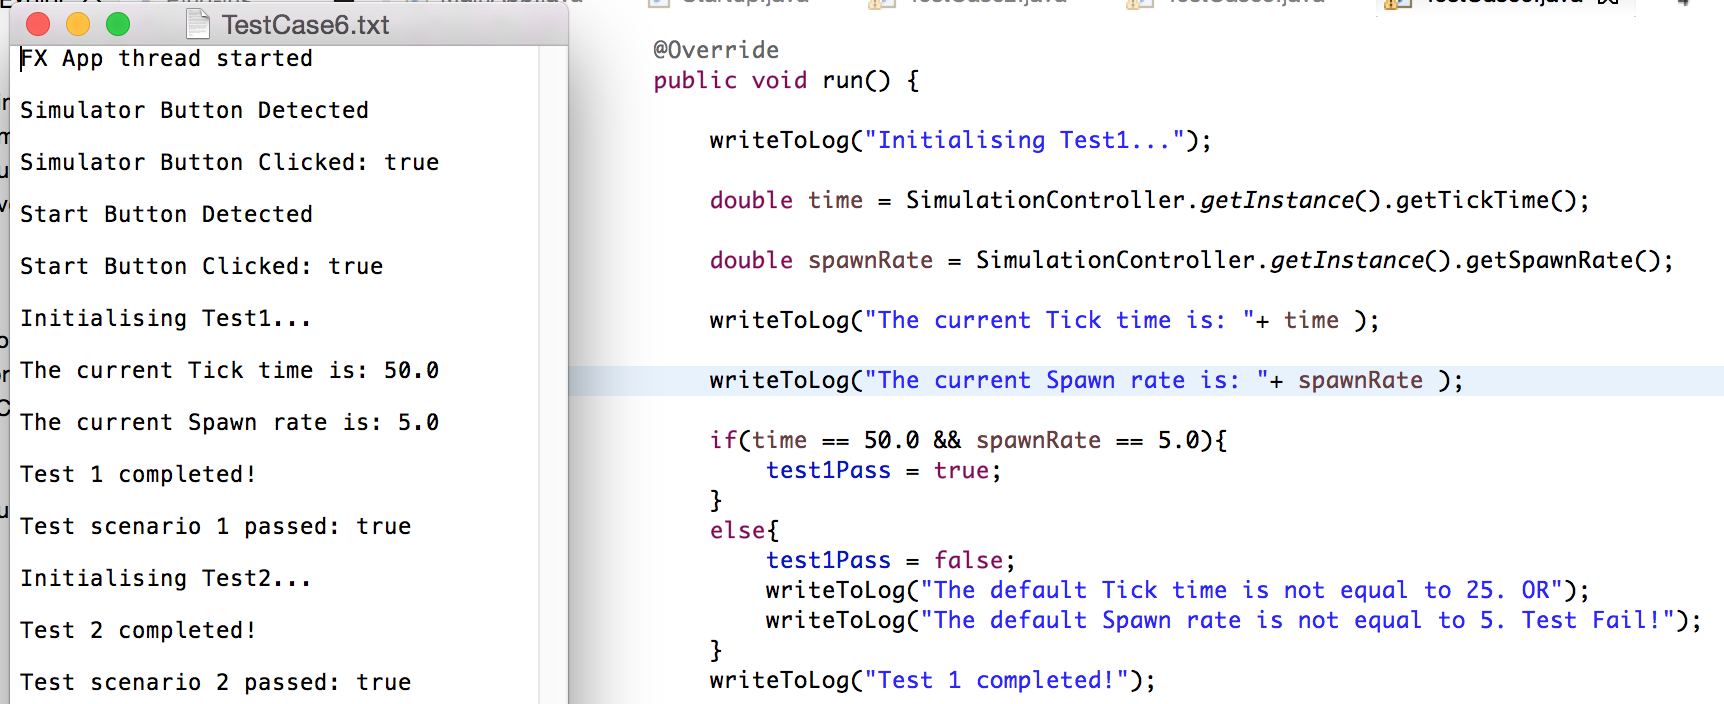
\includegraphics[width=\textwidth]{img/testCase.png}
                \caption{A log is produced after a test execution}
        \label{fig:testCase}
        \end{center}
\end{figure}


Within the framework of testing we also produced a test case table where a formal record is kept for all test cases, detailing the features that were under test. An illustration is shown in figure ~\ref{fig:testCaseTable}.  As incremental changes were made throughout the development, this helped us to define a consistency when every time a test case is executed, that is, the outcome should match the expected result as described.  Furthermore, regression test is a formal method to track the changes throughout a development. due to the constraint of this project, regression test became an impractical option, we hope that test case table would be helpful in the future serving to achieve this purpose.

\begin{figure}[h]
        \begin{center}
                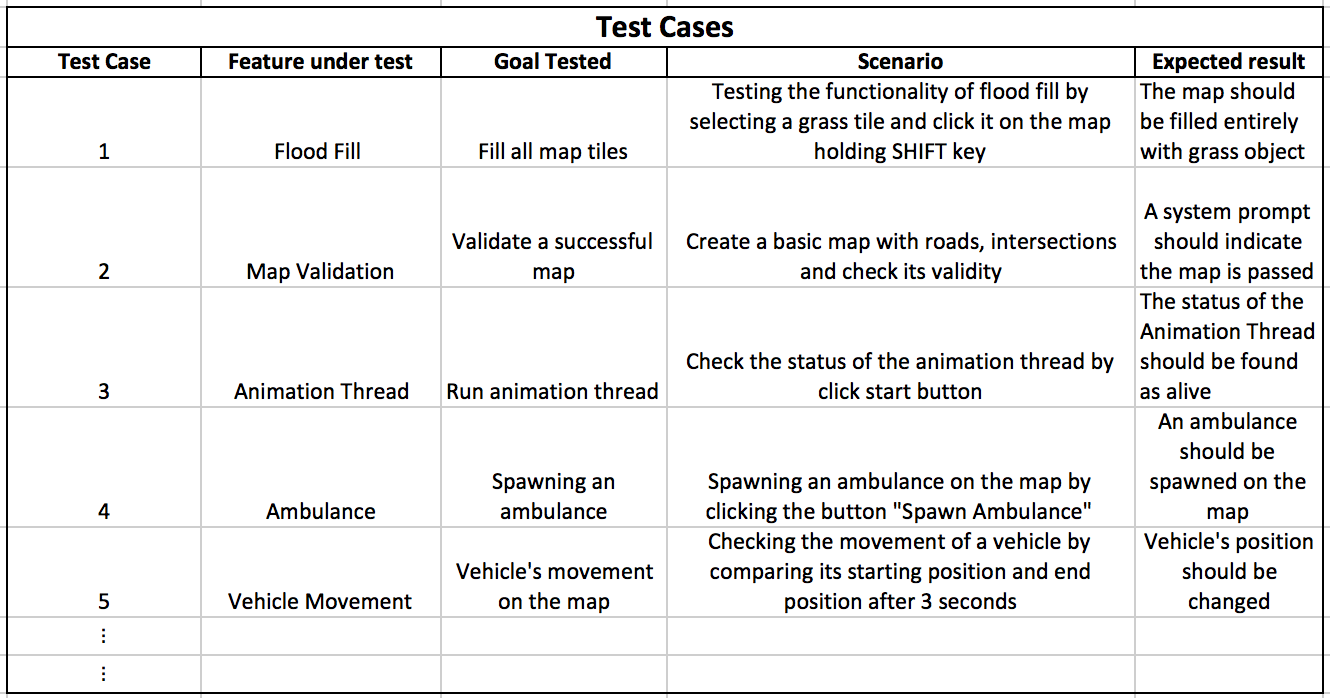
\includegraphics[width=\textwidth]{img/testCaseTable.png}
                \caption{A snippet of test case table}
        \label{fig:testCaseTable}
        \end{center}
\end{figure}

In addition, we also looked at the organisation of our code to further assess the code quality. To do so, we used a commercial tool which helps to picture the system architecture for easy assessment. We produced diagrams such as architectural dependencies, heat maps, UML Class Diagrams, as well as metric reports to give us a visual representation on the internal intricacies of the software. We then fed back the analysis to the development team in order for changes to take place accordingly. For instance, the heat map gave an indication on the level of \textit{lineCount} against \textit{maxCyclomaticComplexity}, as shown in figure ~\ref{fig:heatmap}. The bigger the shape is, the more lines of codes have been written for a class. The colour depth of a shape indicates its maximum complexity. An example of the usefulness of this approach was that we were able to identify the \textit{maxCyclomaticComplexity} for the \textit{Car} class as being 58 and were able to reduce it to 21 for the final version.     

\begin{figure}[h]
        \begin{minipage}{\textwidth}
                \begin{center}
                                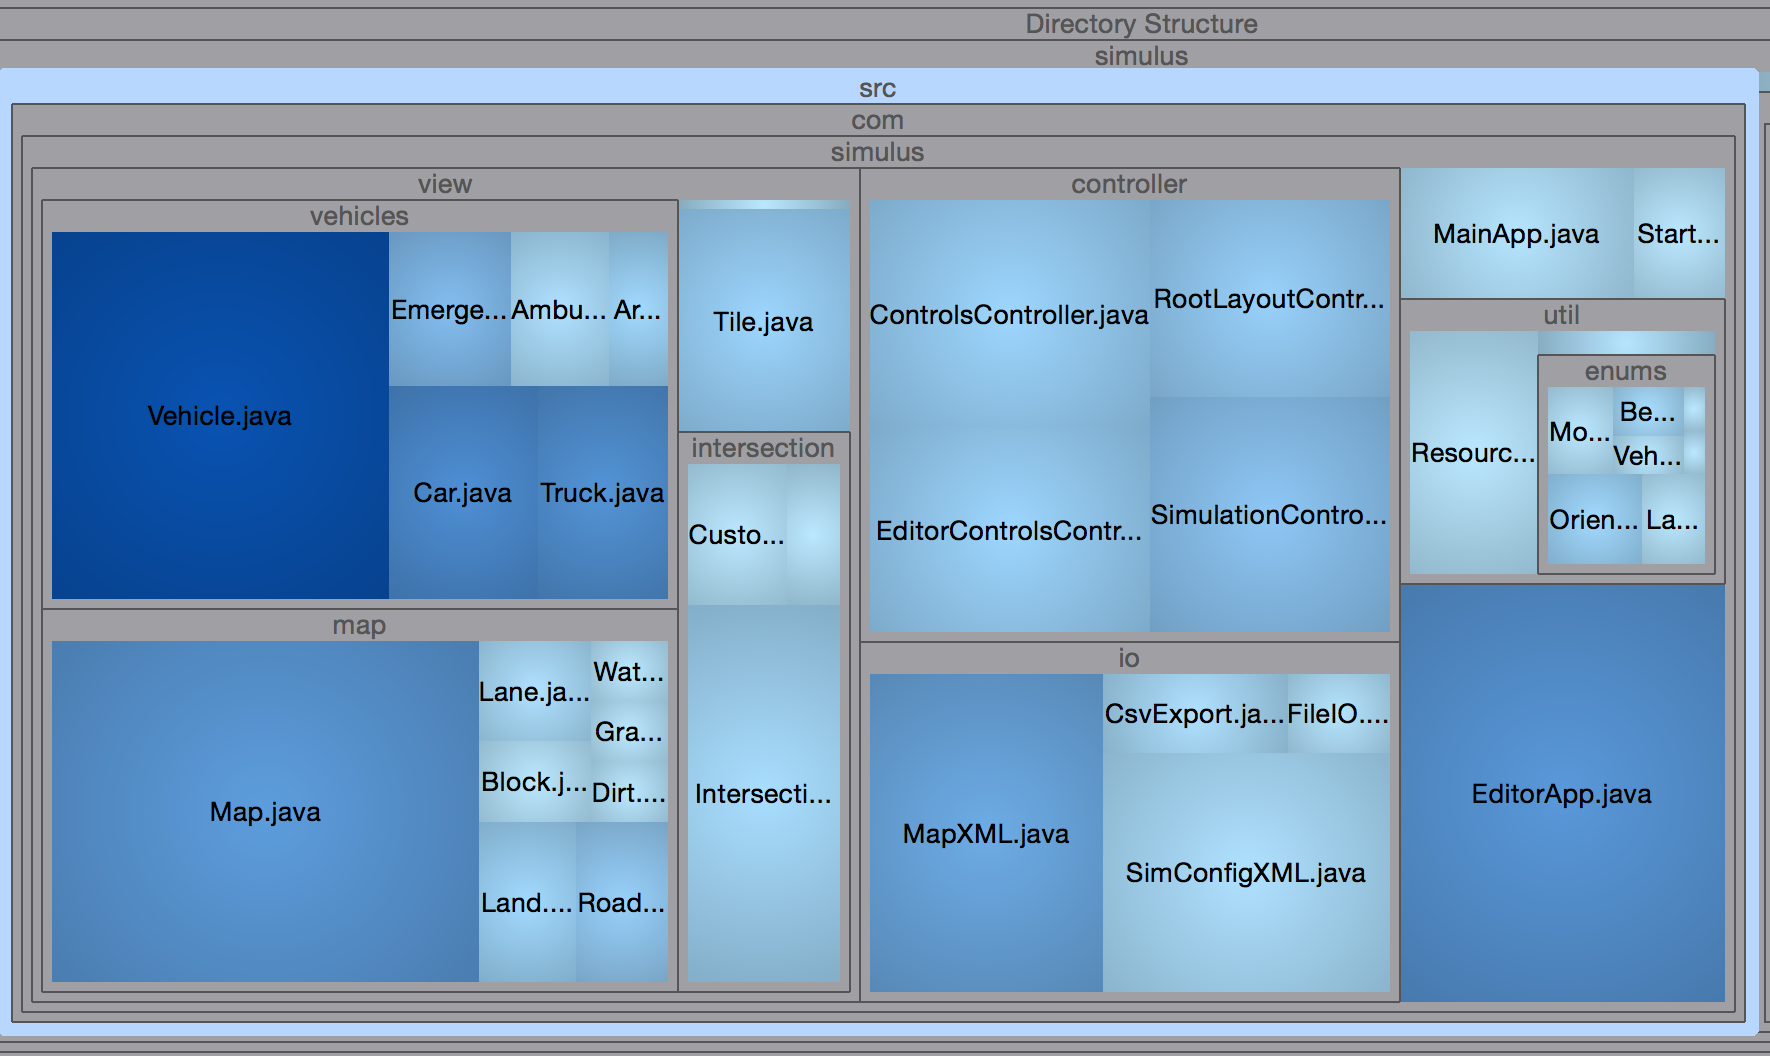
\includegraphics[width=80mm,keepaspectratio ]{img/heatmap.png}
                        \caption{Heat Map for the final version of the software}
                        \label{fig:heatmap}     
                \end{center}
        \end{minipage}
\end{figure}

Figure ~\ref{fig:archIntDependency} illustrates the architectural dependency of our final product. We assured that the outcome was representative of the requirement and design, though only a small portion of bi-directional calls were made internally. In most cases, the architecture is preserved with uni-flow calls. There was no cluster found overall in this project, and so the architecture can therefore be described as clean, depicted in the figure \ref{fig:archIntDependency}. 

\begin{figure}[h]
        \begin{center}
                        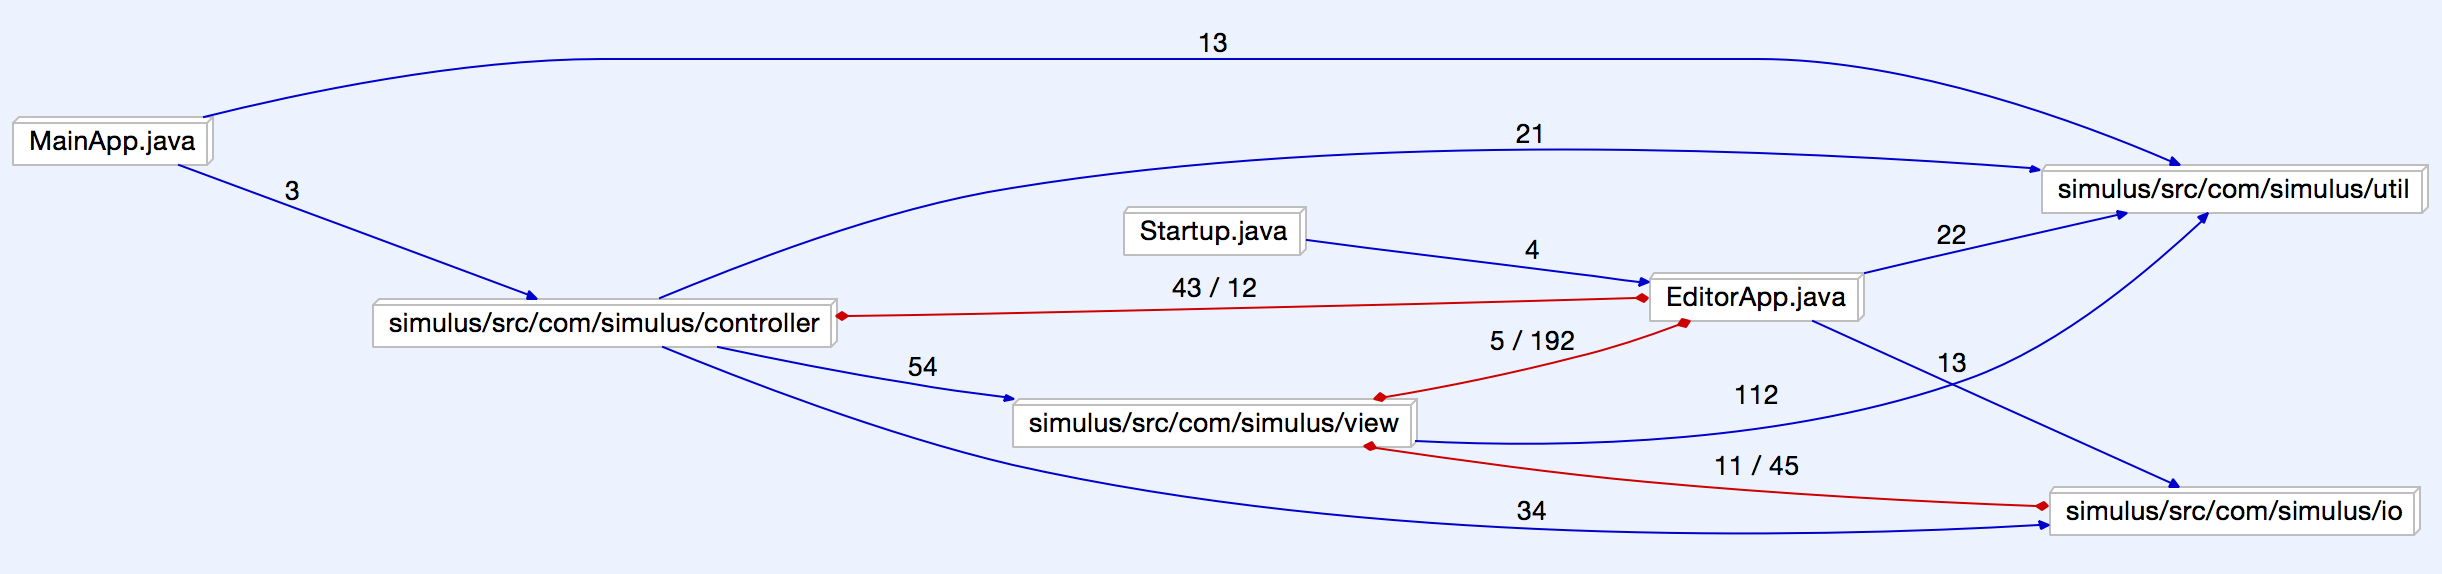
\includegraphics[width=\textwidth]{img/archIntDependency.png}
                \caption{Architecture Internal Dependency}
        \label{fig:archIntDependency}
        \end{center}
\end{figure}



\clearpage